\documentclass{beamer}
%
% Choose how your presentation looks.
%
% For more themes, color themes and font themes, see:
% http://deic.uab.es/~iblanes/beamer_gallery/index_by_theme.html
%
\mode<presentation>
{
  \usetheme{default}      % or try Darmstadt, Madrid, Warsaw, ...
  \usecolortheme{whale} % or try albatross, beaver, crane, ...
  \usefonttheme{default}  % or try serif, structurebold, ...
  \setbeamertemplate{navigation symbols}{}
  \setbeamertemplate{caption}[numbered]
} 

\usepackage[english]{babel}
\usepackage[utf8x]{inputenc}
\usepackage{makecell}
\usepackage{listings}

\title{Quantum A-Star Search}
\subtitle{Presenting a Novel Grover's Based Approach to Optimal Path Findi}
\author{Sam Bieler, Michael Tylko, Eli Shieber}
\institute{ES 170 | Professor Pri}
\date{May 8, 2019}

\begin{document}

\begin{frame}
  \titlepage
\end{frame}

% Uncomment these lines for an automatically generated outline.
%\begin{frame}{Outline}
%  \tableofcontents
%\end{frame}

\begin{frame}{Optimal Pathfinding}

\begin{block}{Problem Statement}
\begin{itemize}
  \item Given a set of nodes, $N$, a set of edges, $E$, a start node, $S$, and a goal node, $F$, what is the optimal route to traverse from start to goal?
  \item Let $f: E \rightarrow \mathbb{R}$ represent a function from edge to edge cost.
  \item Let $e_{ij}$ be the edge between node $i$ and node $j$.
  \item Our goal is then to find a path, $P = (e_{Si},...,e_{jF})$, for which we minimize the objective:
  $$ \sum_{e_{ij} \in P} f(e_{ij}) $$
\end{itemize}
\end{block}
\end{frame}

\begin{frame}{Grid World Problem Set Up}

\begin{block}{Grid World}
\begin{itemize}
  \item We frame the graph for this path finding problem by establishing a grid 
\end{itemize}
\end{block}
\end{frame}

\begin{frame}{Classical A-Star Search}

\begin{block}{Individual Possessions as a Markov Chain}
\begin{itemize}
  \item Each possession is comprised of a set of discrete events such as passes, fouls, shot attempts, and turnovers.
  \item We make the assumption that our  system adheres to the Markov property as the state transition probabilities only depend on the system’s current state.
  \item 36-state Markov chain: 1 Team state, 5 player possession states, 25 player action states (5 for each), 3 scoring states, 1 offensive rebound, and 1 final end of possession.
\end{itemize}
\end{block}
\end{frame}





\begin{frame}{Controlled Z-Gate Implementation}

\begin{block}{4 Qubit Case}
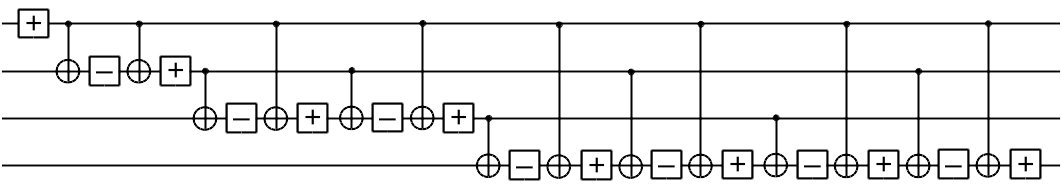
\includegraphics[width=11cm]{4qubitcontrolledzgate.jpg}
\end{block}

\begin{block}{The Pattern}
\begin{itemize}
  \item 0
  \item 0,1,0
  \item 0,1,0,2,0,1,0
  \item 0,1,0,2,0,1,0,3,0,1,0,2,0,1,0
\end{itemize}
\end{block}

\end{frame}


\begin{frame}{Controlled Z-Gate Implementation Continued}[fragile]
\begin{block}{The Code}
\end{block}
\end{frame}

\end{document}
